\documentclass[11pt]{article}
\usepackage[a4paper]{geometry}
\geometry{verbose,tmargin=2cm,bmargin=2cm,lmargin=2cm,rmargin=2cm}
  
\usepackage{fontspec}
\defaultfontfeatures{Ligatures=TeX}

%\setmainfont{Linux Libertine O}
%\setmonofont{Monaco}
    
\setlength{\parindent}{0cm}
  
\usepackage{float}
\usepackage{graphicx}

\usepackage{hyperref}
\usepackage{url}
\usepackage{xcolor}
\usepackage{amsmath}

\usepackage{minted}
%\newminted{scilab}{breaklines,fontsize=\footnotesize}
\newminted{scilab}{breaklines}

\definecolor{mintedbg}{rgb}{0.95,0.95,0.95}
\usepackage{mdframed}

\BeforeBeginEnvironment{minted}{\begin{mdframed}[backgroundcolor=mintedbg]}
\AfterEndEnvironment{minted}{\end{mdframed}}

\begin{document}

\title{Tugas Besar TF2202}
\date{}
\maketitle

test

\begin{scilabcode}
function [a,b] = func1(c,d)
  // Test comment
endfunction
\end{scilabcode}

\section{Soal 1}

Misalkan $y(t)$ menyatakan suatu fungsi dari variabel independen $t$.
$y'(t)$ dan $y''(t)$ secara berturut-turut melambangkan turunan pertama dan
kedua dari $y$ terhadap $t$.

Selesaikan ODE berikut ini
\begin{equation}
y''(t) + y(t) = 0
\end{equation}
dengan syarat awal:
\begin{equation}
y(0) = 0, \hspace{1cm} y'(0) = 1
\end{equation}
dengan menggunakan metode Euler dan predictor-corrector Euler.

Perhatikan bahwa solusi analitik dari permasalahan di atas adalah:
\begin{equation}
y(t) = \sin(t)
\end{equation}

SOLUSI

Dengan menggunakan notasi berikut:
\begin{equation}
y_1 \equiv y, \hspace{1cm} y_2 \equiv y'
\end{equation}

\begin{figure}[H]
\centering
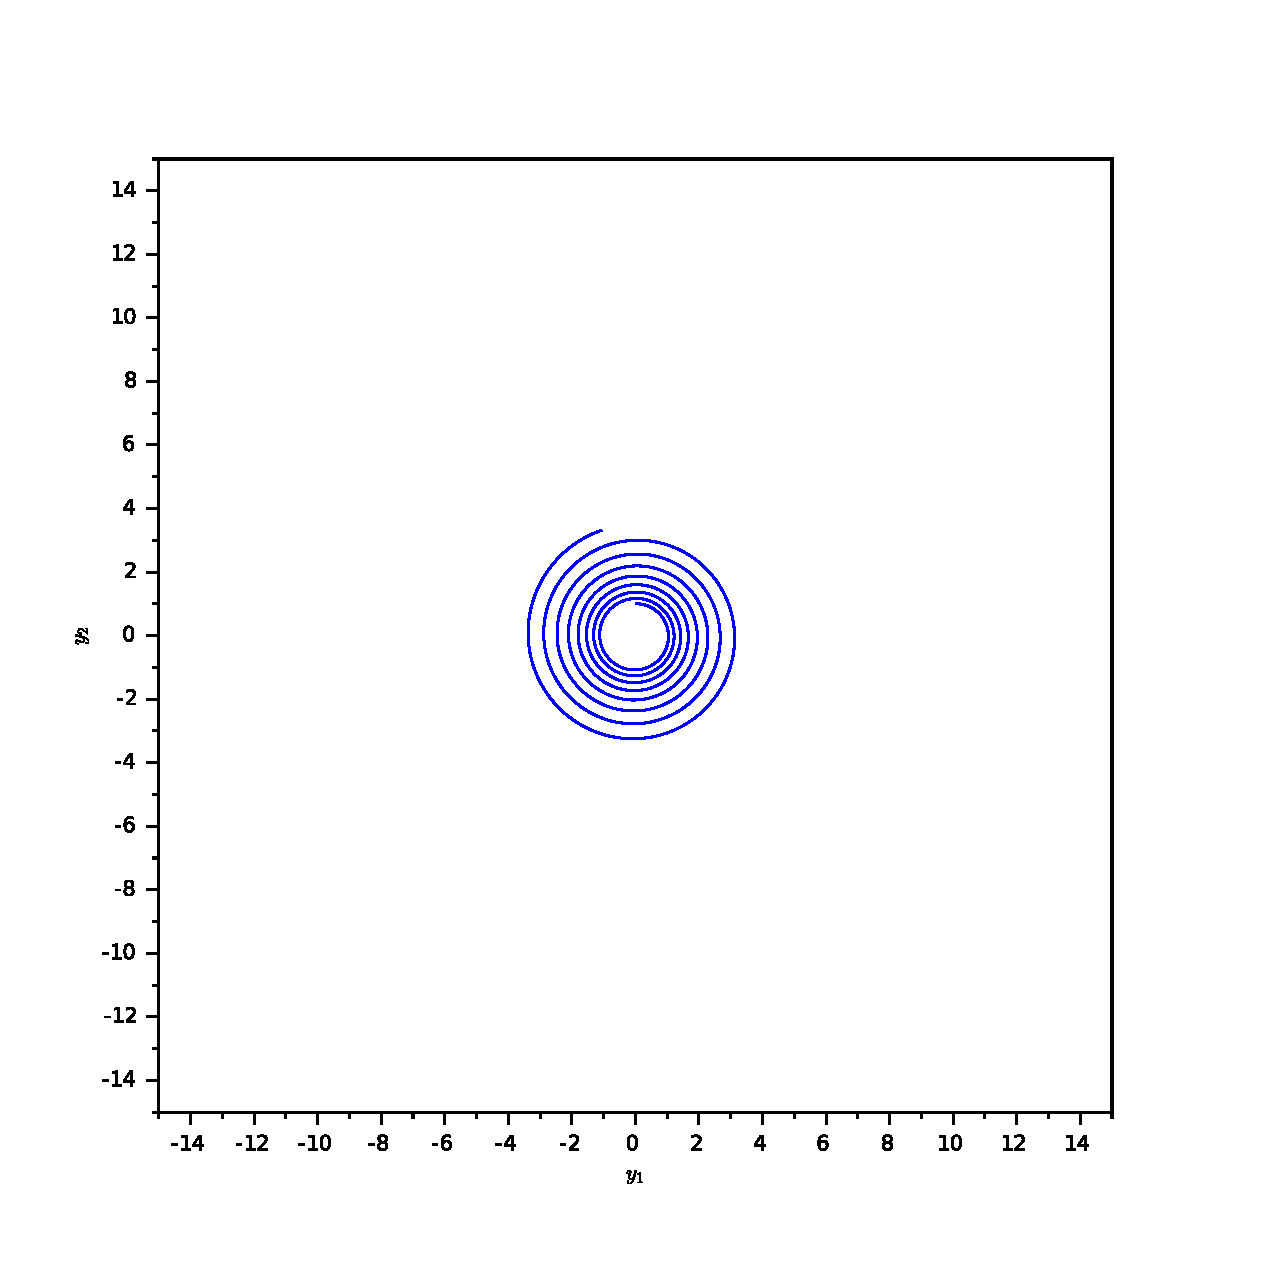
\includegraphics[scale=0.4]{images/soal_01_ode_euler_y1_y2.pdf}
\par
\end{figure}

\begin{figure}[H]
\centering
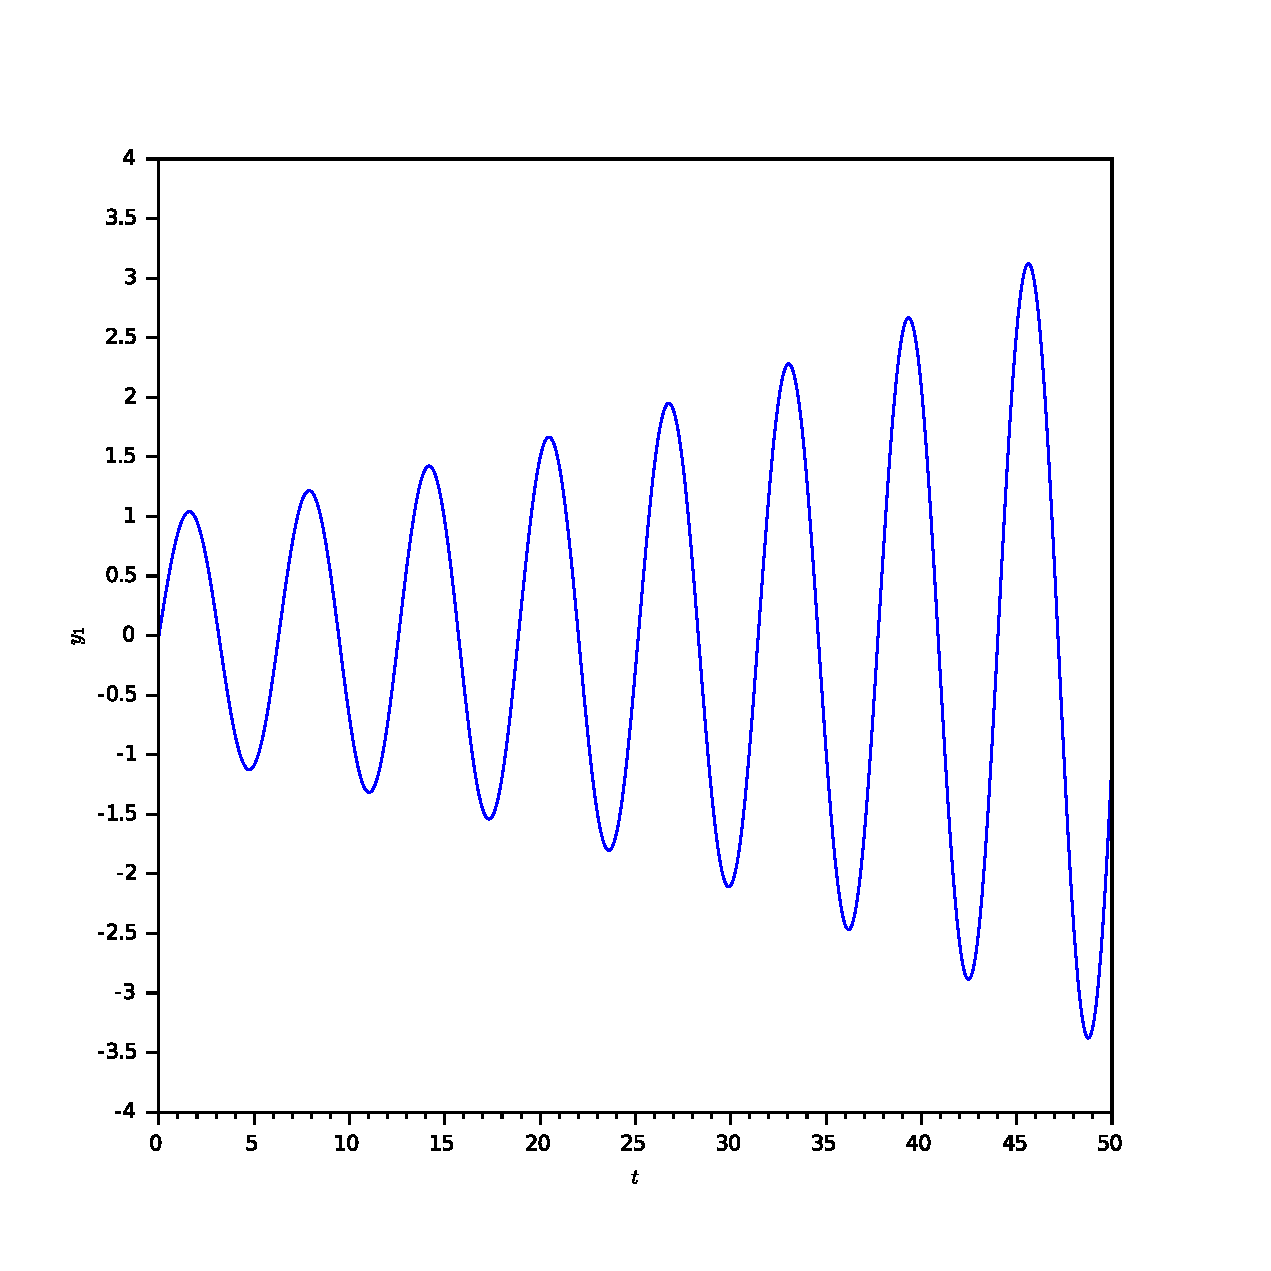
\includegraphics[scale=0.4]{images/soal_01_ode_euler_t_y1.pdf}
\par
\end{figure}

\end{document}